%%%%%%%%%%%%%%%%%%%%%%%%%%%%%%%%%%%%%%%%%%%%%%%%%%%%%%%%%%%%%%%%%%%%%%
% Lớp 11 | Hàm số lượng giác và phương trình lượng giác | Hàm số lượng giác và đồ thị
% Dạng 1D1?4-8: Toán thực tế áp dụng hàm số lượng giác
% Số câu: 30  (sinh tự động bởi tach_cau.py; từ nay thầy sửa trực tiếp file này)
%%%%%%%%%%%%%%%%%%%%%%%%%%%%%%%%%%%%%%%%%%%%%%%%%%%%%%%%%%%%%%%%%%%%%%

%%%%%%%%%%%%%%%% ĐÚNG/SAI %%%%%%%%%%%%%%%%

% nguồn: Ok_dungsai_lop11_Lan2
\begin{ex}%[1D1H4-8]%[ma:eab62aae]
	Chiều cao so với mực nước biển trung bình tại thời điểm $t$  (giây) của mỗi cơn sóng được cho bởi hàm số $h(t)=75\sin \left(\dfrac{\pi t}{8}\right)$, trong đó $h(t)$ được tính bằng centimét.
	\choiceTF{\True Chiều cao của sóng  tại các thời điểm $5$ giây bằng $69{,}3$ (cm)}
		{\True Chiều cao của sóng tại các thời điểm  $20$ giây bằng $75$ (cm)}
		{Trong $30$ giây đầu tiên (kể từ mốc  $t=0$ giây), thời điểm để sóng đạt chiều cao lớn nhất $6$ giây}
		{Trong $30$ giây đầu tiên (kể từ mốc $t=0$ giây), thời điểm để sóng đạt chiều cao  lớn nhất $18$ giây. (Tất cả kết quả được làm tròn đến hàng phần mười)}
	 \loigiai{
		\begin{itemchoice}
			 \itemch \textbf{Đúng.}\\
			Khi $t=5$, ta có $h(5)=75\sin  \left(\dfrac{\pi\cdot 5}{8}\right)\approx 69{,}3$ (cm).
			\itemch \textbf{Đúng.}\\ 
			Khi $t=20$, ta có $h(20)=75\sin \left(\dfrac{\pi \cdot 20}{8}\right)=75$  (cm).
			 \itemch \textbf{Sai.}\\
			Ta có $\sin  \left(\dfrac{\pi t}{8}\right)\le 1\Rightarrow 75\sin \left(\dfrac{\pi t}{8}\right)\le 75$ hay $h(t) \le 75$.
			Giá trị lớn nhất của $h(t)$ là $75$, khi đó $\sin \left(\dfrac{\pi t}{8}\right)=1\Rightarrow \dfrac{\pi t}{8}=\dfrac{\pi}{2}+k2\pi\ (k\in \mathbb{Z})$.\\ 
			Suy ra  $t=4+16k\ (k\in \mathbb{Z})$.
			\itemch  \textbf{Sai.}\\
			Vì $t\in  [0; 30]\Rightarrow t\in \{4; 20\}$ (ứng với $k$ bằng $0$ và $1$).
			Vậy tại các thời điểm $4$ giây hoặc $20$ giây (trong $30$ giây đầu tiên) thì cơn sóng đạt  chiều cao cực đại (là $75$ (cm)).
		\end{itemchoice}
	} 
\end{ex}

% nguồn: Ok_dungsai_lop11_Lan2
\begin{ex}%[1D1H4-8]%[ma:7cb49f56]
	Giả sử vận tốc $v$  (tính bằng lít/giây) của luồng khí trong một chu kì hô hấp (tức là thời gian từ lúc bắt đầu của một nhịp thở đến khi bắt đầu của nhịp thở tiếp theo) của một người nào đó ở trạng thái nghỉ ngơi được cho bởi công thức $v=0{,}85\sin \dfrac{\pi t}{3}$, trong đó $t$ là thời gian (tính bằng giây).
	Xét tính đúng sai của các mệnh đề  sau
	\choiceTF{\True Vận tốc của luồng khí tại giây thứ ba  là $0$ lít/giây}
		{Thời gian của một chu kì hô hấp đầy đủ  là $3$ giây}
		 {\True Số chu kì hô hấp trong một phút của người đó là $10$}
		{Thời điểm lần đầu vận tốc của luồng khí  đạt giá trị lớn nhất là $t=0{,}5$ giây}
	 \loigiai{
		Vận tốc  của luồng khí tại giây thứ ba là $v=0{,}85\sin \dfrac{\pi\cdot 3}{3}=0$ lít/giây. \\
		Hàm số  $v=0{,}85\sin \dfrac{\pi t}{3}$ tuần hoàn với chu kì $T=\dfrac{2\pi}{\dfrac{\pi}{3}}=6$. \\
		Số chu kì hô hấp trong  một phút ($60$ giây) của người đó là $60: 6=10$. \\
		Thời điểm lần đầu vận tốc của luồng khí đạt giá trị lớn nhất là $t=\dfrac{\pi}{2}: \dfrac{\pi}{3}=1{,}5$ giây. 
		\begin{itemchoice}
			\itemch \textbf{Đúng.}\\ 
			Vận tốc của luồng khí  tại giây thứ ba là $0$ lít/giây.
			\itemch \textbf{Sai.}\\ 
			Thời gian của một chu kì hô hấp đầy đủ là  $6$ giây
			\itemch \textbf{Đúng.}\\ 
			Số chu kì hô hấp  trong một phút của người đó là $10$.
			 \itemch \textbf{Sai.}\\
			Thời  điểm lần đầu vận tốc của luồng khí đạt giá trị lớn nhất là $t=1{,}5$ giây.
		\end{itemchoice}
	} 
\end{ex}

% nguồn: Ok_dungsai_lop11_Lan2
\begin{ex}%[1D1H4-8]%[ma:5ab677cc]
	Giả sử  khi một cơn sóng biển đi qua một cái cọc ở ngoài khơi, chiều cao của nước được mô hình hóa bởi hàm số $h(t)=90\cos \left(\dfrac{\pi}{10} t\right)$, trong đó $h(t)$ là độ cao tính bằng centimét trên mực nước biển trung bình tại thời điểm $t$ giây.
	\choiceTF{\True Độ cao trên mực nước biển  trung bình tại thời điểm $t=5$ giây là $0$ (cm)}
		{\True  Chu kì của sóng là $20$ (giây)}
		{Chiều cao của sóng (khoảng  cách theo phương thẳng đứng giữa đáy và đỉnh của sóng) là $90$ (cm)}
		{\True  Số lần xuất hiện đỉnh sóng trong một phút là $3$}
	\loigiai{ 
		Độ cao trên  mực nước biển trung bình tại thời điểm $t=5$ giây là $h(5)=90\cos \left(\dfrac{\pi}{2}\right)=0$ (cm).
		Hàm số $h(t)=90\cos \left(\dfrac{\pi}{10} t\right)$ tuần hoàn với chu kì $T=\dfrac{2\pi}{\dfrac{\pi}{10}}=20$ nên chu kì của sóng  là $20$ giây.
		Giá trị lớn nhất và giá trị nhỏ nhất của hàm số $h(t)=90\cos \left(\dfrac{\pi}{10} t\right)$ lần lượt là $90$  và $-90$ nên chiều cao của sóng là $90-(-90)=180$ (cm).
		Số lần xuất hiện đỉnh  sóng trong một phút (60giây) là $60: 20=3$.
		\begin{itemchoice}
			\itemch  \textbf{Đúng.}\\
			Độ cao trên mực nước biển trung bình tại thời điểm  $t=5$ giây là $0$ (cm).
			\itemch \textbf{Đúng.}\\ 
			Chu  kì của sóng là $20$ (giây).
			 \itemch \textbf{Sai.}\\
			Chiều cao của sóng là $180$  (cm).
			\itemch  \textbf{Đúng.}\\
			Số lần xuất hiện đỉnh sóng  trong một phút là $3$.
		\end{itemchoice}
	} 
\end{ex}

% nguồn: Ok_dungsai_lop11_Lan2
\begin{ex}%[1D1V4-8]%[ma:94f3e67f]
	Chiều cao so với mực nước biển trung bình tại thời điểm $t$ (giây) của mỗi cơn sóng được cho bởi hàm số $h(t)=75\sin \left(\dfrac{\pi t}{8} \right)$, trong đó  $h(t)$ được tính bằng centimét.
	 \choiceTF
		{\True Chiều cao của sóng  tại các thời điểm $5$ giây bằng $69{,}3$\,cm}
		{\True Chiều  cao của sóng tại các thời điểm $20$ giây bằng $75$\,cm}
		{Trong $30$  giây đầu tiên (kể từ mốc $t=0$ giây), thời điểm để sóng đạt chiều cao lớn nhất $6$ giây}
		{Trong $30$ giây đầu tiên (kể từ mốc $t=0$ giây), thời điểm để sóng đạt chiều cao lớn nhất $18$  giây (Tất cả kết quả được làm tròn đến hàng phần mười)}
	 \loigiai{
		\begin{itemchoice}
			\itemch Khi $t=5$ ta có $h(5)=75\sin  \left(\dfrac{\pi\cdot 5}{8} \right)\approx 69{,}3$\,cm.
			\itemch  Khi $t=20$ ta có $h(20)=75\sin \left(\dfrac{\pi\cdot 20}{8} \right)=75$\,cm.
			\itemch Ta có $\sin \left(\dfrac{\pi t}{8} \right)\le 1\Rightarrow 75\sin \left(\dfrac{\pi t}{8} \right)\le 75$ hay  $h(t)\le 75$.\\
			Giá trị lớn nhất của $h(t)$ là $75$  khi đó \allowdisplaybreaks
			\begin{eqnarray*}
				&&\sin \left(\dfrac{\pi  t}{8} \right)=1\\
				 &\Leftrightarrow& \dfrac{\pi t}{8}=\dfrac{\pi}{2}+k2\pi\\
				&\Leftrightarrow& t=4+16k\left(k\in  \mathbb{Z}\right).
			\end{eqnarray*}
			Vì $t\in [0;30]\Rightarrow t\in \{4;20\}$ (ứng với $k$ bằng $0$ và $1$).\\ 
			Vậy tại các thời điểm $4$ giây hoặc $20$ giây (trong $30$ giây đầu tiên) thì cơn sóng đạt chiều cao cực đại là  $75$\,cm.
			 \itemch
		\end{itemchoice}
	} 
\end{ex}


%%%%%%%%%%%%%%%% TRẢ LỜI NGẮN %%%%%%%%%%%%%%%%

% nguồn: Ok_TraLoiNgan_Lop11_Lan1
\begin{ex}%[1D1N4-8]%[ma:e3937c7d]
	Một vật  dao động điều hòa và chuyển động theo phương trình li độ $x=5\cos \left(10\pi t+\dfrac{\pi}{6} \right)$ cm. Tìm li độ của vật tại thời điểm $t=0{,}05s$.
	\shortans{-2,5} 
	 \loigiai{
		Tại thời điểm  $t=0{,}05s$ ta có $x=5\cos \left(10\pi\cdot 0{,}05+\dfrac{\pi}{6} \right)=-2{,}5$ cm.
	 }
\end{ex}

% nguồn: Ok_TraLoiNgan_Lop11_Lan2
\begin{ex}%[1D1N4-8]%[ma:68f3ae4e]
	Mỗi ngày, người ta quan sát thấy mặt trời mọc đầu tiên tại Mỹ là tại vùng núi đảo ở Maine. Thời điểm mặt trời mọc được biểu diễn theo công thức $t(m)=1{,}665\sin (m+3)+5{,}485$, với $t$ là thời điểm (được tính từ nửa đêm) và $m$ là tháng (tính từ tháng $1$). Hãy cho biết vào tháng $3$ thì mặt trời mọc lúc mấy giờ (kết quả để ở  dạng thập phân, làm tròn đến hàng phần trăm)?
	\shortans{5,02} 
	 \loigiai{
		Ta  có $t(3)=1{,}665\sin (3+3)+5{,}485\approx 5{,}0197\approx 5{,}02$ giờ. \\
		Vậy vào tháng $3$ thì mặt trời mọc lúc khoảng $5{,}02$  giờ.
	} 
\end{ex}

% nguồn: Ok_TraLoiNgan_Lop11_Lan1
\begin{ex}%[1D1H4-8]%[ma:d22612e1]
	Hằng ngày mực nước của con kênh lên xuống theo thủy triều. Độ sâu $h$ (mét) của mực nước trong kênh được tính tại thời điểm $t$ (giờ) trong một ngày bời công thức $h=3 \cos \left(\dfrac{\pi t}{8}+\dfrac{\pi}{4}\right)+12$.  Mực nước của kênh cao nhất khi nào?
	 \shortans{14}
	\loigiai{Mực nước của kênh cao nhất khi $h$ lớn nhất khi 
		 $$\cos \left(\frac{\pi t}{8}+\frac{\pi}{4}\right)=1 \Leftrightarrow \frac{\pi t}{8}+\frac{\pi}{4}=k 2 \pi \Leftrightarrow t+2=16k.$$
		Do  $0<t\le 24$ và $k \in \mathbb{Z}$ nên $\heva{&k=1\\&t=14.}$\\
		Vậy mực nước  của kênh cao nhất khi $t=14$ giờ.
	} 
\end{ex}

% nguồn: Ok_TraLoiNgan_Lop11_Lan1
\begin{ex}%[1D1H4-8]%[ma:07afb212]
	Hằng ngày mực nước con kênh lên xuống theo thủy triều. Độ sâu $ h$ (mét) của mực nước trong kênh được tính tại thời điểm $t$ giờ ($0\le t\le24$) trong một ngày bởi công thức $ h=3\cos\left(\dfrac{\pi t}{8}+\dfrac{\pi}{4}\right)+12$. Biết mực nước của kênh cao nhất khi $t=t_0$, tính  giá trị của $t_0$.
	 \shortans{14}
	 \loigiai{
		Mực nước cao  nhất của kênh đạt được khi
		\begin{align*}
			\cos \left(\frac{\pi t_0}{8}+\frac{\pi}{4}\right)=1 \Leftrightarrow \frac{\pi t_0}{8}+\frac{\pi}{4}= k2\pi, k\in\mathbb{Z} \Leftrightarrow  t_0=16k -2, k\in \mathbb{Z}.
		\end{align*}
		Do $0\le t_0\le 24$ nên $k=1$ và  $t_0=14$.
	} 
\end{ex}

% nguồn: Ok_TraLoiNgan_Lop11_Lan2
\begin{ex}%[1D1H4-8]%[ma:f1761dd0]
	Huyết áp của mỗi người thay đổi trong ngày. Giả sử huyết áp tâm trương (tức là áp lực máu lên thành động mạch khi tim giãn ra) của một  người nào đó ở trạng thái nghỉ ngơi tại thời điểm $t$ được cho bởi công thức
	$$ 
	B(t)=a+b \sin \dfrac{\pi  t}{12}, (a, b>0),
	 $$
	trong đó $t$ là số giờ tính từ lúc nửa đêm và $B(t)$ tính bằng mmHg (milimét thủy ngân). Biết huyết áp tâm trương thấp nhất là $78$ mmHg và huyết áp tâm trương  lớn nhất là $92$ mmHg. Hỏi huyết áp tâm trương của người đó vào thời điểm $2$ giờ $30$ phút chiều bằng bao nhiêu (kết quả để ở dạng thập phân, làm tròn đến hàng phần chục)?
	 \shortans{80,7}
	 \loigiai{
		Vi $a, b>0$ và $-1\leq \sin \dfrac{\pi t}{12}\leq 1$ nên $\max\limits_{t\in[0; 24]} B(t)=a+b$, $\min\limits_{t\in[0;  24]} B(t)=a-b$ nên ta có $$\heva{&a+b=92 \\ & a-b=78}\Leftrightarrow\heva{&a=85 \\& b=7.}$$
		Tại thời điểm $2$ giờ $30$ phút chiều thì thời gian $t=14{,}5$  giờ. \\
		Huyết áp tâm trương của người đó là $B(14{,}5)=85+7\sin  \dfrac{\pi \cdot 14{,}5}{12}\approx 80{,}7\mathrm{mmHg}$.
	} 
\end{ex}

% nguồn: Ok_TraLoiNgan_Lop11_Lan2
\begin{ex}%[1D1H4-8]%[ma:355812dd]
	Mực nước lên xuống của  thủy triều trong một ngày tại một cửa biển được tính theo công thức $y=\sin \left(\dfrac{\pi}{180}(x+73) \right)+1$ với $x$ là giờ $(0\leq x \leq 24)$, $y$ tính theo đơn vị $m$ so với mực nước biển.
	Hỏi vào lúc $17$  h thì mực nước ở độ cao bao nhiêu mét so với mực nước biển?
	\shortans{2} 
	 \loigiai{
		Thay $x=17$ vào công thức $y=\sin \left(\dfrac{\pi}{180}(x+73) \right)+1$ ta có $y=\sin \left(\dfrac{\pi}{180}(17+73) \right)+1=2$.  \\
		Vậy vào  lúc $x=17$ thì mực nước ở độ cao $2$ m so với mực nước biển.
	 }
\end{ex}

% nguồn: Ok_TraLoiNgan_Lop11_Lan2
\begin{ex}%[1D1H4-8]%[ma:56eab8d6]
	Hàng ngày, mực nước của một con kênh lên xuống theo thủy triều. Độ sâu $h(\mathrm{~cm})$ của mực nước trong kênh tính theo thời gian $t$ (giờ) trong một ngày $(0\leq t \leq 24)$ cho bởi công  thức $h=3\cos \left(\dfrac{\pi t}{12}+\dfrac{\pi}{3}\right)+10$. Hỏi vào thời điểm nào trong ngày, mực nước của con kênh đạt độ cao lớn nhất?
	\shortans{20} 
	 \loigiai{
		Ta có  $3\cos \left(\dfrac{\pi t}{12}+\dfrac{\pi}{3}\right)+10\leq 13$. \\
		Mà $3\cos \left(\dfrac{\pi t}{12}+\dfrac{\pi}{3}\right)+10=13\Leftrightarrow \cos \left(\dfrac{\pi t}{12}+\dfrac{\pi}{3}\right)=1\Leftrightarrow \dfrac{\pi t}{12}+\dfrac{\pi}{3}=k 2\pi \Leftrightarrow t=24k-4(k \in \mathbb{Z})$.  \\
		Từ đó có $0\leq 24k-4\leq  24\Leftrightarrow \dfrac{1}{6}\leq k \leq \dfrac{7}{6}\Rightarrow k=1\Rightarrow t=20$. \\
		Vậy vào thời điểm $20$ h trong ngày, mực nước của  con kênh đạt độ cao lớn nhất là $13(\mathrm{~cm})$.
	} 
\end{ex}

% nguồn: Ok_TraLoiNgan_Lop11_Lan2
\begin{ex}%[1D1H4-8]%[ma:326b4fd5]
	Số giờ có ánh sáng mặt trời của một thành phố X ở vĩ độ $40^\circ $ bắc trong ngày thứ $t$ của một năm không nhuận được cho bởi hàm số $d(t)=3\sin\left[\dfrac{\pi}{182}\left(t-80\right)\right]+12,$ $\,t\in\mathbb{Z}\text{,}$ $0<t\leq 365$. Vào ngày nào trong năm thì thành phố X có nhiều giờ có ánh sáng mặt trời nhất? 
	 \shortans{171}
	\loigiai{ 
		Vì $-1\le\sin\alpha\leq 1$, $\forall\alpha  $ nên ta có $d(t)=3\sin\left[\dfrac{\pi}{182}\left(t-80\right)\right]+12\leq 3\cdot1+12=15$.\\
		Suy ra $d{(t)_{\max}}=15$ đạt được khi $$\sin\left[\dfrac{\pi}{182}\left(t-80\right)\right]=1\Leftrightarrow\dfrac{\pi}{182}\left(t-80\right)=\dfrac{\pi}{2}+k2\pi\Leftrightarrow t=171+364k,\, k\in\mathbb{Z}.$$ 
		Vì $0<t\leq 365$ nên ta  có $0<171+364k\leq 365\Rightarrow\dfrac{-171}{364}<k\le\dfrac{194}{364}$ do $k\in\mathbb{Z}$ nên $k=0$.\\
	Vậy vào ngày thứ $171$ trong  năm thì thành phố X có nhiều giờ có ánh sáng mặt trời nhất.}
\end{ex}

% nguồn: Ok_TraLoiNgan_Lop11_Lan2
\begin{ex}%[1D1H4-8]%[ma:8cae57f6]
	Số giờ có ánh sáng mặt trời của  một thành phố X ở vĩ độ $40^0$ bắc trong ngày thứ $t$ của một năm không nhuận được cho bởi hàm số $d(t)=3\sin\left[\dfrac{\pi}{182}\left(t-80\right)\right]+12$, $t\in\mathbb{Z}$, $0<t\leq 365$. Vào ngày nào trong năm thì thành phố X có ít giờ có ánh sáng mặt trời nhất?
	\shortans{353} 
	 \loigiai{
		 Ta có $\sin\left[\dfrac{\pi}{182}\left(t-80\right)\right]
		\geq-1$, $\forall t\Rightarrow d(t)\geq 3\cdot\left(-1\right)+12=9$.  Dấu \lq\lq$=$\rq\rq\, xảy ra khi\\
		$$\sin\left[\dfrac{\pi}{182}\left(t-80\right)\right]=-1\Leftrightarrow\dfrac{\pi}{182}\left(t-80\right)=-\dfrac{\pi}{2}+k2\pi\Leftrightarrow t-80=-91+364k\Leftrightarrow t=-11+364k,  k\in\mathbb{Z}.$$
		Mà $0<t\leq 365\Rightarrow 0<-11+364k\leq  365\Leftrightarrow\dfrac{11}{364}<k\le\dfrac{376}{364}\Leftrightarrow k=1\,\left(\text{do}k\in\mathbb{Z}\right)\Rightarrow t=353$.\\
	Vậy thành phố X có ít giờ có ánh sáng mặt trời nhất vào ngày $353$  trong năm.}
\end{ex}

% nguồn: Ok_TraLoiNgan_Lop11_Lan2
\begin{ex}%[1D1H4-8]%[ma:5bc8643d]
	Giả sử số miligam của các chất ô nhiễm trong một mét khối không khí trong một tháng tại một thành phố công nghiệp được xác định bởi công thức $$P(t)=a+b \sin \left[\dfrac{2 \pi}{7}\left(t-\dfrac{37}{12}\right)\right], (a, b>0), $$ trong đó $t$ là số ngày kể từ ngày thứ Bảy của tuần đầu tiên. Biết chất ô nhiễm trong một mét khối không khí cao nhất là $50$ miligam và thấp nhất là $20$ miligam. Hỏi trong ngày thứ Hai của tuần thứ $2$, ngày thứ Tư của tuần thứ $3$ và ngày thứ Ba của tuần thứ $4$ và ngày thứ Sáu  của tuần thứ $4$ của tháng thì số miligam chất ô nhiễm nhiều nhất bằng bao nhiêu (kết quả để ở dạng thập phân, làm tròn đến hàng đơn vị)?
	 \shortans{46}
	\loigiai{ 
		Vì $a, b>0$ và $-1\leq \sin \left[\dfrac{2\pi}{7}\left(t-\dfrac{37}{12}\right)\right] \leq  1$ nên $\heva{&P(t)_{\max}=a+b \\& P(t)_{\min}=a+b}\Rightarrow\heva{&a+b=50\\ & a-b=20}\Leftrightarrow\heva{&a=35\\& b=15.}$\\
		Suy ra  $P(t)=35+15\sin \left[\dfrac{2\pi}{7}\left(t-\dfrac{37}{12}\right)\right], (a, b>0)$. \\
		Số miligam của ngày thứ Hai của tuần thứ $2$ là $P(2) \approx  23$. \\
		Số miligam của ngày thứ  Tư của tuần thứ $3$ là $P(11) \approx 46$. \\
		 Số miligam của ngày thứ Ba của tuần thứ $4$ là $P(17) \approx 34$. \\
		Số miligam của ngày thứ Sáu của  tuần thứ $4$ là $P(20)=43$. \\
		Vậy số  miligam chất ô nhiễm nhiều nhất khoảng $46$ miligam.
	} 
\end{ex}

% nguồn: Ok_TraLoiNgan_Lop11_Lan2
\begin{ex}%[1D1H4-8]%[ma:bd93e788]
	Hằng ngày mực nước của  con kênh lên xuống theo thủy triều. Độ sâu $h$ (mét) của mực nước trong kênh được tính tại thời điểm $t$ (giờ) trong một ngày bởi công thức $$h=3\cos\left(\dfrac{\pi t}{8}+\dfrac{\pi}{4}\right)+12.$$ Mực nước của kênh cao nhất khi $t$ bằng bao nhiêu?
	\shortans{14} 
	\loigiai{ 
		Mực nước  của kênh cao nhất khi độ sâu của mực nước trong kênh lớn nhất.\\
		Ta có $-1\le\cos\left(\dfrac{\pi t}{8}+\dfrac{\pi}{4}\right)\leq 1$ $\Leftrightarrow $ $9\leq 3\cos\left(\dfrac{\pi t}{8}+\dfrac{\pi}{4}\right)+12\leq  15$.\\
		Nên  $\max h=15$ khi $\cos\left(\dfrac{\pi t}{8}+\dfrac{\pi}{4}\right)=1\Leftrightarrow t=-2+16k, k\in\mathbb{Z}$.\\
		Trong 1 ngày có 24  giờ nên $0\le-2+16k\leq 24$ $\Leftrightarrow\dfrac{1}{8}\leq k\le\dfrac{26}{16}$.\\
	Vì $k\in\mathbb{Z}$ nên $k=1$ $\Rightarrow t=14$  (giờ).}
\end{ex}

% nguồn: Ok_TraLoiNgan_Lop11_Lan1
\begin{ex}%[1D1V4-8]%[ma:542182a0]
	Số giờ có ánh sáng của thành phố $T$ ở vĩ độ $40^{^\circ}$ bắc trong ngày thứ $t$ của một năm không nhuận được cho bởi hàm số $d(t)=3\cdot \sin \left[\dfrac{\pi}{182} (t-80)\right]+12$ với $t\in \mathbb{Z}$ và $0< t\le 365$. Bạn An muốn đi  tham quan thành phố $T$ nhưng lại không thích ánh sáng mặt trời, vậy bạn An nên chọn đi vào ngày nào trong năm để thành phố $T$ có ít giờ có ánh sáng mặt trời nhất?
	\shortans{353} 
	 \loigiai{
		 Do
		 $$
		\begin{aligned}
			\sin \left[\dfrac{\pi}{182} (t-80)\right]\ge-1 &\Rightarrow  3\cdot \sin \left[\dfrac{\pi}{182} (t-80)\right]\ge-3\\
			&\Rightarrow 3\cdot \sin \left[\dfrac{\pi}{182} (t-80)\right]+12\ge 9\Rightarrow  d(t)\ge 9.
		\end{aligned}
		 $$
		Vậy thành phố  $T$ có ít giờ có ánh sáng mặt trời nhất khi và chỉ khi:
		\[\sin \left[\dfrac{\pi}{182} (t-80)\right]=-1\Leftrightarrow \dfrac{\pi}{182}  (t-80)=-\dfrac{\pi}{2}+k2\pi
		\] 
		\[\Leftrightarrow t-80=182\left(-\dfrac{1}{2}+2k\right)\Leftrightarrow t=364k-11,k\in  \mathbb{Z}.
		\] 
		Mặt khác $0\le 364k-11\le 365\Leftrightarrow \dfrac{11}{364} \le  k\le \dfrac{376}{364} \Leftrightarrow k=1($ do $k\in \mathbb{Z})$. Nên
		\[t=364-11=353\] 
		 Vậy thành phố $T$ có ít giờ ánh sáng Mặt Trời nhất là $9$ giờ khi $t=353$, tức là vào ngày thứ $353$ trong năm.
	 }
\end{ex}

% nguồn: Ok_TraLoiNgan_Lop11_Lan1
\begin{ex}%[1D1V4-8]%[ma:36aded96]
	Giả sử khi một cơn sóng biển đi qua một cái cọc ở ngoài khơi, chiều cao của nước được mô hình hoá bởi hàm số $h(t)=90 \cos \left(\dfrac{\pi}{10}t\right)$, trong đó $h(t)$ là độ  cao tính bằng centimét trên mực nước biển trung bình tại thời điểm $t$ giây. Tìm chiều cao của sóng (cm) (là khoảng cách theo phương thẳng đứng giữa đáy và đỉnh của sóng).\\
	 \shortans{180}
	\loigiai{ 
		Ta có $-90 \leq 90 \cos \left(\dfrac{\pi}{10} t\right) \leq  90$.\\
	Suy ra chiều cao của sóng là $90- (-90)  =180$ (cm). }
\end{ex}

% nguồn: Ok_TraLoiNgan_Lop11_Lan1
\begin{ex}%[1D1V4-8]%[ma:6a5922b2]
	\immini{Một con lắc lò xo dao động điều hòa quanh vị trí cân bằng theo phương trình $y=25\sin 4\pi t$, trong  đó $y$ được tính bằng centimét còn thời gian $t$ được tính bằng giây. Khoảng cách giữa điểm cao nhất và thấp nhất của con lắc bằng bao nhiêu centimét? }
	{\begin{tikzpicture}[scale=.75,font=\footnotesize,line join=round,line cap=round,>=stealth]
		\node[rectangle,draw,minimum width=8mm,minimum height = 6mm] (a) at  (0,2) {};
		 \node[rectangle,draw,fill=teal,minimum width=8mm,minimum height = 6mm] (b) at (0,0) {};
		\draw[decoration={aspect=0.3,segment length=1.5mm,amplitude=3mm,coil},decorate]  (0,5) -- (a);
		\draw[dashed,decoration={aspect=0.3,segment length=3mm,amplitude=3mm,coil},decorate] (0,2.25)  -- (b);
		\fill [pattern = north east lines] (-1,5) rectangle  (1.3,5.2);
		\draw (-1,5)  -- (1.3,5);
		\draw (-3.5,1)--(1,1); 
		\draw (-3.5,1)--(1,1); 
		\node () at (-2.4,1.2){V{ị} tr{í} c{â}n b{ằ}ng}; 
		\draw  (0.4,2)--(1,2);
		 \draw[<->] (0.6,1)--(0.6,2) node[midway,right]{$y>0$};
		\draw[<->] (0.6,1)--(0.6,-.25)  node[midway,right]{$y<0$};
	\end{tikzpicture}
	} 
	\shortans{50} 
	\loigiai{ 
		Do $-1\le \sin 4\pi t\le 1$  nên $-25\le 25\sin 4\pi t\le 25$, hay $-25\le y\le 25$.\\
		 Vậy khoảng cách giữa điểm cao nhất và thấp nhất của con lắc là $25-(-25)=50$ (cm).
	} 
\end{ex}

% nguồn: Ok_TraLoiNgan_Lop11_Lan1
\begin{ex}%[1D1V4-8]%[ma:59ec1bae]
	Hằng ngày, mực nước của một con kênh lên xuống theo thuỷ triều. Độ sâu $h$ (m) của mực nước trong kênh tính theo thời gian $t$ (giờ) trong một ngày $(0 \leq t<24)$ cho bởi công thức $h=\cos \left(\dfrac{\pi t}{6}+2 \pi\right)+5$. Hỏi trong ngày vị trí nước xuống mức thấp nhất trễ nhất  là mấy giờ?
	 \shortans{21}
	 \loigiai{
		Với mọi $0 \leq t<24$  ta có
		$$-1\leq \cos \left(\dfrac{\pi t}{6}+2 \pi\right)\leq  1 \Leftrightarrow 4\leq \cos \left(\dfrac{\pi t}{6}+2 \pi\right)+5\leq 6.$$
		Mực nước thấp nhất của  kênh $h=4$ (m) khi
		\begin{align*}
			\cos \left(\dfrac{\pi t}{6}+2 \pi\right)=-1 \Leftrightarrow \dfrac{\pi t}{6}+2\pi=-\dfrac{\pi  }{2}+k2\pi \Leftrightarrow t=-15+12k, k\in \mathbb{Z}.
		\end{align*}
		Do $0\le t\le 24$ nên  $k=2$, $t=9$ và $k=3$, $t=21$.\\
		Vậy lúc $9$ và $21$ giờ mực  nước kênh là thấp nhất và $h=4$ (m). Vậy mực nước thấp trễ nhất lúc $21$ giờ.
	} 
\end{ex}

% nguồn: Ok_TraLoiNgan_Lop11_Lan1
\begin{ex}%[1D1V4-8]%[ma:67ed31ca]
	\immini[thm]{Người ta nghiên cứu sự sinh trưởng và phát triển của một loại sinh vật $A$ trên một hòn đảo thì thấy sinh vật $A$ phát triển theo quy luật $$s(t)=a+b\sin\dfrac{\pi t}{18},\  a,b\in\mathbb{R}$$ với $s(t)$ là số lượng sinh vật $A$ sau $t$ năm và có đồ thị như hình vẽ.}
	{ 
	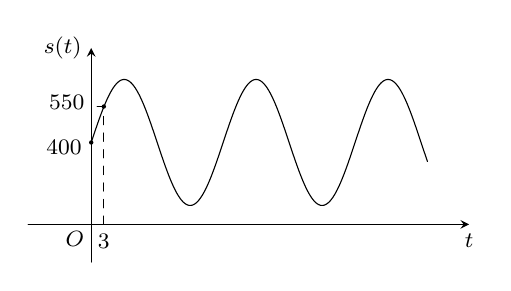
\begin{tikzpicture}[scale=0.8,font=\footnotesize,line join=round,line cap=round,>=stealth]
			\draw[->]  (-1,0)--(6,0) node [below]{$t$};
			\draw[->] (0,-0.6)--(0,2.8) node [left]{$s  (t)$};
			\node at (0,0) [below left=-1pt]{$O$}; 
			 \draw plot[samples=300,domain=0:1.7*pi](\x,{1.3+sin (3*\x r)});
			\fill (0,1.3) circle (1pt) node[shift={(-170:10pt)}]{$400$}; 
			\fill (0.2,1.27+sin 0.6r) circle  (1pt);
			\draw[dashed] (0.2,0)  node[shift={(-90:6pt)}]{$3$}|-(0,1.27+sin 0.6r) node[shift={(170:9pt)}]{$550$};
		\end{tikzpicture}
	 }
	Hỏi số lượng sinh vật  $A$ được nhiều nhất bao nhiêu con?
	 \shortans{700}
	 \loigiai{
		Dựa vào đồ thị ta  thấy $\heva{
		&s(0)=400\\ 
		&s(3)=550\\}\Rightarrow\heva{ 
		&a=400\\ 
		 &b=550.\\}$\\
		Suy ra  $s(t)=400+300\sin\dfrac{\pi}{18}t$.\\
		Ta có $$-1\leq \sin\dfrac{\pi}{18}t\leq 1\Leftrightarrow-300\leq 300\sin\dfrac{\pi}{18}t\leq 300\Leftrightarrow 100 \leq  400+ 300\sin\dfrac{\pi}{18}t\leq 700\ (\forall t\geq 0).$$
		Vậy số lượng sinh vật  nhiều nhất là $700$ con.
	 }
\end{ex}

% nguồn: Ok_TraLoiNgan_Lop11_Lan1
\begin{ex}%[1D1V4-8]%[ma:dfc0e75c]
	\immini{Khi đu quay hoạt động, vận tốc theo phương ngang của một cabin $M$ phụ thuộc vào góc lượng giác $\alpha = \left(Ox,OM\right)$ theo hàm số $v_x = 0{,}5\sin\alpha$ (m/s).  Giá trị lớn nhất của $ v_x $ là
	 }{\resizebox{!}{4.5cm}{
	\begin{tikzpicture}[font=\small,line join=round,line cap=round,>=stealth]
			\tikzset{declare function={g=0;}} 
			 \coordinate (O) at (0,0);
			 \pgfmathsetmacro{\gx}{60-g};
			 \draw (O) circle (4.4)
				(O)  circle (3.53);
			\foreach \t in {0,1,...,11}{ 
				\draw[very thick,fill] (O)--(g+30*\t:4.4) circle  (0.06);
				\begin{scope}[shift={(g+30*\t:4.4)}]
				\draw[fill=teal] (-0.27,0)--(0.27,0)--(0.36,-0.18)--(-0.36,-0.18)--cycle 
				 (0.32,-0.18)--(0.32,-0.54)
				(-0.32,-0.18)--(-0.32,-0.54) 
				 (-0.4,-0.54)--(0.4,-0.54)--(0.27,-1)--(-0.27,-1)--cycle;
				\end{scope}}
			\draw[fill=gray!70!yellow]  (0.2,0)--(2.35,-5.53)--(3.65,-5.53)--(3.65,-6.02)--(1.95,-6.02)--(0,-0.85)--(-1.95,-6.02)--(-3.65,-6.02)--(-3.65,-5.53)--(-2.35,-5.53)--(-0.2,0)--cycle;
			\draw[fill=gray!10!yellow] (O) circle  (0.34);
			 \draw[fill] (-5,-5.85)--(0,-5.85) circle (0.08)--(6.4,-5.85);
			 \draw[->] (-5,0)--(6.7,0) node [below]{\color{black}$x$};
			\path 
				(3.82,2.22) coordinate (M) 
				($(M)-(1.8,0)$) coordinate  (N)
				 ($(N)+(0,2.5)$) coordinate (P);
			\fill[black] (M) circle (1pt)  node[above right]{$M$};
			\fill[black]  (N) circle (0pt) node[below left]{$\overrightarrow{v}_x$};
			\fill[black] (P) circle (0pt)  node[above]{$\overrightarrow{v}$};
			 \fill[black] (O) circle (1pt);
			\fill[black] (O)+(-90:0.3) circle (0pt) node[below]{$O$}; 
			\draw[->] (M)--(N); 
			\draw[->] (M)--(P); 
			\draw[dashed]  (N)--(P);
			\draw  (O)--(M);
			\draw[->] (O)+(0:0.8) arc (0:30:0.8) node[below right]{$\alpha$}; 
			 \draw pic[draw,angle radius = 4mm] {right angle=O--M--P};
		\end{tikzpicture}
	}} 
	 \shortans{0,5}
	 \loigiai{ Với mọi $ \alpha $ ta có\\
		$ -1\le \sin\alpha \le 1 \Rightarrow -0{,}5\le 0{,}5\sin\alpha \le 0{,}5 \Rightarrow -0{,}5 \le  v_x \le 0{,}5$.\\
		Vậy giá trị lớn  nhất của $v_x$ là $0{,}5$ (m/s).
	 }
\end{ex}

% nguồn: Ok_TraLoiNgan_Lop11_Lan1
\begin{ex}%[1D1V4-8]%[ma:3467e127]
	Cho vận tốc $v$ (cm/s) của một con lắc đơn theo thời gian $t$ (giây) được cho bởi công thức $v=-4\sin\left(1{,}5t+\dfrac{\pi}{3}\right)$ với $0\le t \le 2$. Xác định thời điểm vận tốc con lắc bằng $2$ cm/s.  (Làm tròn kết quả đến hàng chục).
	 \shortans{1,7}
	 \loigiai{
		Ta có 
		\begin{eqnarray*}
			& & -4\sin\left(1{,}5t+\dfrac{\pi}{3}\right)=2\\ 
			 &\Leftrightarrow & \sin\left(1{,}5t+\dfrac{\pi}{3}\right)=\dfrac{-1}{2}\\
			&\Leftrightarrow & \hoac{&1{,}5t+\dfrac{\pi}{3}=\dfrac{-\pi}{6}+k2\pi \\ & 1{,}5t+\dfrac{\pi}{3}=\dfrac{7\pi}{6}+k2\pi}\\ 
			&\Leftrightarrow  & \hoac{& t=\dfrac{-\pi}{3}+\dfrac{k4\pi}{3} \\ & t= \dfrac{5\pi}{9} + \dfrac{k4\pi}{3}} (k\in\mathbb{Z}).
		\end{eqnarray*}
		TH1: $ t=\dfrac{-\pi}{3}+\dfrac{k4\pi}{3}$, $0\le t  \le 2 $
		$ \Rightarrow 0\le \dfrac{-\pi}{3}+\dfrac{k4\pi}{3} \le  2 \Rightarrow \dfrac{1}{4}\le k \le \dfrac{6+\pi}{4\pi} \approx 0{,}73$.\\
		Mà $  k\in \mathbb{Z} $ suy ra $ k\in \varnothing$.\\
		TH2:  $ t= \dfrac{5\pi}{9} + \dfrac{k4\pi}{3}, 0\le t\le 2 $
		$ \Rightarrow  0\le \dfrac{5\pi}{9} + \dfrac{k4\pi}{3} \le 2 \Rightarrow \dfrac{-5}{3} \le t \le \dfrac{18-5\pi}{12\pi}\approx 0{,}06 $.\\
		Mà  $ k\in \mathbb{Z} $ suy ra $ k=0 \Rightarrow t=\dfrac{5\pi}{9}\approx 1{,}7 $ (giây).\\
	} 
\end{ex}

% nguồn: Ok_TraLoiNgan_Lop11_Lan2
\begin{ex}%[1D1V4-8]%[ma:12541626]
	Số giờ có ánh sáng mặt trời của Thủ đô Hà Nội năm 2018 được cho bởi công thức $y=3\sin \left(\dfrac{\pi}{180}(x+60) \right)+13$ với $1\leq x \leq 365$ là số thứ tự của ngày trong năm. Ngày nào của năm 2018 thì số giờ có ánh sáng  mặt trời của Hà Nội lớn~nhất?
	 \shortans{30}
	 \loigiai{
		Để số giờ có ánh sáng mặt trời lớn nhất thì hàm số $y=3\sin \left(\dfrac{\pi}{180}(x+60) \right)+13$ đạt giá trị  lớn nhất. \\ Khi đó $\sin \left(\dfrac{\pi}{180}(x+60) \right)=1\Leftrightarrow x=30+k 360(k \in \mathbb{Z})$. \\
		Vì $1\leq x \leq  365$ nên ta có
		$1\leq 30+k  360\leq 365\Leftrightarrow-0{,}08\leq k \leq 0{,}93\Rightarrow k=0$. \\
		Do đó $x=30$ (tháng đầu tiên của năm) 
	 }
\end{ex}

% nguồn: Ok_TraLoiNgan_Lop11_Lan2
\begin{ex}%[1D1V4-8]%[ma:13d69c2e]
	\immini[thm]{ 
	Một cái guồng nước có vành kim loại ngoài cùng là một đường tròn tâm $O$, bán kính là $4$ m. Xét chất điểm $M$ thuộc đường tròn đó và góc $\alpha=(OA, OM)$. Giả sử mực nước lúc đang xét là tiếp xúc với đường tròn $(O; 4)$ và guồng nước quay  theo chiều dương (ngược chiều kim đồng hồ).
	Biết rằng guồng nước quay hết một vòng sau $40$ giây ($t=0$ giây khi điểm $M$ trùng $A$). Hỏi thời điểm nào (trong $1$ vòng quay đầu tiên) thì  điểm $M$ ở vị trí cao nhất so với mặt nước?}{
	\begin{tikzpicture}[line join = round,line cap = round,>=stealth,font=\footnotesize,scale=.5]
			\foreach  \i in {0,1,...,40}
			 \draw[gray] (0,0)--(\i*10:5);
			 \draw[line width=3pt,green!50!black] (0,0) circle (5cm);
			 \draw[gray] (0,0) circle (4.5cm);
			 \draw[gray] (0,0) circle (4cm);
			\draw[gray] (0,0)  circle (3.5cm);
			\draw[green!60!black,line width=1pt]  (5,0) coordinate (A)--(0,0) coordinate (O)--++(60:5) coordinate (M) node[above right]{$M$};
			\draw[->] pic [draw,angle radius = 9 mm] {angle = A--O--M}; 
			\draw[red] (.7,.45) node{$\alpha$}; 
			\fill  (M) circle (3pt);
			\fill (0,0)  node[below left]{$O$} circle (3pt);
			\fill (5,0) node[above right] {$A$} circle (2pt); 
			 \draw[->] (-6,0)--(6,0) node[below]{$x$};
			 \draw[->] (0,-6)--(0,6) node[right]{$y$};
		\end{tikzpicture}
	 }
	 \shortans{10}
	 \loigiai{
		Ta có $h(x)=4+4 \sin \alpha$.  \\
		Khi $M$ ở vị trí cao nhất so với mặt nước (tức là $h(x)=8$) thì $\sin \alpha=1 \Rightarrow  \alpha=\dfrac{\pi}{2}$ (vì chỉ xét $1$ vòng quay đầu tiên). \\
		Thời gian thực hiện của guồng nước là  $t=\dfrac{\dfrac{\pi}{2}\cdot 40}{2 \pi}=10$ (giây).
	} 
\end{ex}


%%%%%%%%%%%%%%%% TỰ LUẬN %%%%%%%%%%%%%%%%

% nguồn: Ok_TuanLuan_Toan11_Lan2
\begin{ex}%[1D1H4-8]%[ma:f164b73b]
	Trong hình dưới đây, một chiếc máy bay $A$ bay ở độ cao $500$ (m) theo một đường thẳng đi ngang qua phía trên trạm quan sát $T$ ở mặt đất. Hình chiếu vuông  góc của $A$ lên mặt đất là $H$ và $\alpha$ là góc lượng giác $(Tx, TA)$, ($0<\alpha<\pi$). Hãy cho biết với $\dfrac{\pi}{6}<\alpha<\dfrac{2\pi}{3}$ thì $x_H$ nằm trong khoảng nào (\textit{làm tròn kết quả đến hàng phần mười})?
	\begin{center}
		\begin{tikzpicture}[line join = round,line cap=round,>=stealth,font=\footnotesize,scale=1]
				 \tikzset{maybay/.pic={
				 \def\dam{1}
				\draw[black,line width=\dam  pt]
					(0.85,4.15) --  (1.2,4.15) -- (1.4,3.7) -- (3.6,3.7)
					..controls +(0:1.2) and +(20:0.85).. (4.7,1.82) -- (2.9,1.82) 
					..controls  +(180:0.9) and +(-48:0.8).. (1.78,3.07)
					 ..controls +(130:0.1) and +(0:0.00).. (1.28,3.1)
					..controls +(180:0.4)  and +(-90:0.05).. cycle
					(3.5,2.3) -- (3.75,2.3) 
					 (2.5,2.95) -- (3.1,2.95)
					 (2.8,3.25) -- (2.8,2.65)
					(2.5,3.7) --  (2.5,4.07) -- (3.26,4.07) -- (3.26,3.77)
					(1.17,4.72) -- (4.62,4.72) -- (4.42,4.42) -- (2.97,4.32)--(1.37,4.42)--cycle 
					 (1.9,0.87) -- (4.6,0.87) -- (5.15,1.2) -- (4.8,1.44) -- (4.5,1.24) -- (1.85,1.24) -- cycle;
				 \foreach \x in {2.9,3.25,3.83,4.2}{
					\draw[line width=\dam  pt] (\x,1.8) -- (\x,1.3);
				 }
				\draw[fill=white,line  width=\dam pt]
					(2.7,4.1) -- (2.7,4.85)..controls +(90:0.2) and +(90:0.2)..  (3.1,4.85) -- (3.1,4.1) -- cycle;
				\draw[line width=\dam  pt,rounded corners=2mm]
					(3.55,3.7)  -- (3.55,2.65) -- (4.95,2.65)
					(3.8,3.4)..controls +(0:0.4) and +(90:0.04).. (4.6,2.9); 
					 }}
				\def\ca{-3} 
				 \path
					(0,0) coordinate (A) 
					(0,\ca)  coordinate (H)
					(4,\ca) coordinate (T); 
				\path 
					(-1.5,0.1)  pic[scale=.2]{maybay};
				\draw[dashed](-3,0)--(4.5,0); 
				 \draw
					 (T)--(A)--(H)
					($(A)!.5!(H)$) node[left]{$500$}; 
				\draw[->](4.5,\ca)--(-3,\ca)  node[above]{$x$};
				 \foreach \x/\g in {A/150,H/-90,T/-90}\fill(\x) circle (1pt)+(\g:.3) node{$\x$};
				\draw pic[draw,angle  radius=3mm,angle eccentricity=1.5,"$\alpha$"] {angle = A--T--H};
			\end{tikzpicture}
	\end{center}
	\loigiai{Ta có  $x_H=500\cot\alpha$.\\
		 Với $\dfrac{\pi}{6}<\alpha<\dfrac{2\pi}{3}$ thì $-\dfrac{\sqrt{3}}{3}<\cot\alpha<\sqrt{3}$ nên $x_H\in\left(-288{,}7; 866\right)$.
	 }
\end{ex}

% nguồn: Ok_TuanLuan_Toan11_Lan2
\begin{ex}%[1D1H4-8]%[ma:a78b090c]
	\immini{ 
	Khi đu quay hoạt động, vận tốc theo phương ngang của một  cabin $M$ phụ thuộc vào góc lượng giác $\alpha=(Ox, OM)$ theo hàm số $v_x=0{,}3\sin\alpha$ (m/s).
	\begin{enumerate}
		 \item Tìm giá trị lớn nhất và giá trị nhỏ nhất của $v_x$.
		\item Dựa vào đồ thị của  hàm số sin, hãy cho biết trong vòng quay đầu tiên ($0\leq\alpha\leq 2\pi$), góc $\alpha$ ở trong các khoảng nào thì $v_x$ tăng.
	\end{enumerate}
	} 
	{ 
	\begin{tikzpicture}[scale=0.5,font=\small,line join=round,line cap=round,>=stealth]
			 \tikzset{declare function={g=0;}}
			\coordinate (O) at  (0,0);
			\coordinate[label=above  right:$A$] (A) at (0:4.4);
			 \coordinate[label=above right:$M$] (M) at (30+g:4.4);
			 \pgfmathsetmacro{\gx}{60-g};
			\coordinate (v)  at ($(M)+(120+g:3.3)$);
			\coordinate  (vx) at ($(M)+(180:3.3*cos \gx)$);
			\draw(O)  circle (4.4)
				(O)  circle (3.53);
			\foreach \t in  {0,1,...,11}{
				\draw[very  thick,fill] (O)--(g+30*\t:4.4) circle (0.06);
				\begin{scope}[shift={(g+30*\t:4.4)}]
				\draw[fill=teal]  (-0.27,0)--(0.27,0)--(0.36,-0.18)--(-0.36,-0.18)--cycle
				 (0.32,-0.18)--(0.32,-0.54)
				 (-0.32,-0.18)--(-0.32,-0.54)
				(-0.4,-0.54)--(0.4,-0.54)--(0.27,-1)--(-0.27,-1)--cycle; 
				\end{scope}}
			 \draw[fill=gray!70!yellow] (0.2,0)--(2.35,-5.53)--(3.65,-5.53)--(3.65,-6.02)--(1.95,-6.02)--(0,-0.85)--(-1.95,-6.02)--(-3.65,-6.02)--(-3.65,-5.53)--(-2.35,-5.53)--(-0.2,0)--cycle;
			 \draw[fill=gray!10!yellow] (O) circle (0.34);
			\draw[fill]  (-5,-5.85)--(0,-5.85) circle (0.08)--(6.4,-5.85);
			\draw[->,red] (-5,0)--(6.7,0)  node [below]{\color{black}$x$};
			\draw[->,red] (M)--(v)  node [left=-2pt]{\color{black}$\vec{v}$};
			\draw[->,red] (M)--(vx)  node [below left=-5pt]{\color{black}$\vec{v}_{\!\!x}$};
			 \draw (O)--(M);
			\draw[dashed,red]  (0,0)--(0,-5.85)
				(v)--(vx); 
			\fill (0,0) circle (0.1); 
			\path pic[draw=red,angle  radius=5]{right angle=v--M--O}
				(O) pic[draw,->,angle radius=16]{angle=A--O--M}  node[shift={(14:23pt)}]{$\alpha$};
			\node  at (O)[below]{$O$};
		\end{tikzpicture}
	 }
	 \loigiai{
		\begin{enumerate}
			\item Do  $-1\leq\sin\alpha\leq 1$ nên $-0{,}3\leq 0{,}3\sin\alpha\leq 0{,}3$.\\
			Vậy giá trị lớn nhất của $v_x$ là $0{,}3$ (m/s) và giá trị nhỏ nhất của $v_x$  là $-0{,}3$ (m/s).
			\item Ta thấy vòng quay  đầu tiên ($0\le\alpha\leq 2\pi$) thì $v_x$ tăng khi $0\le\alpha\leq \dfrac{\pi}{2}$ và $\dfrac{3\pi}{2}\le\alpha\leq 2\pi$.
		\end{enumerate}
	 }
\end{ex}

% nguồn: Ok_TuanLuan_Toan11_Lan2
\begin{ex}%[1D1H4-8]%[ma:3575d48c]
	Giả sử khi một cơn sóng biển đi qua một cái cọc ở ngoài khơi, chiều cao của nước được mô hình hoá bởi hàm số $h(t)=90\cos\left(\dfrac{\pi}{10} t\right), $ trong đó $h(t)$ là độ cao tính bằng centimét trên mực nước biển trung bình  tại thời điểm $t$ giây.
	\begin{enumerate}
		\item Tìm chu kì của  sóng.
		\item Tìm chiều cao của sóng, tức là  khoảng cách theo phương thẳng đứng giữa đáy và đỉnh của sóng.
	\end{enumerate}
	 \loigiai{
		\begin{enumerate}
			 \item Chu kì của sóng là $T=\dfrac{2\pi}{\dfrac{\pi}{10}}=20$ (giây).
			\item Chiều cao của sóng tức là chiều cao của nước đạt được trong một chu kì  dao động.\\
			 Ta có $h(20)=90\cos\left(\dfrac{\pi}{10} \cdot 20\right)=90$\,cm.\\
			Vậy chiều cao  của sóng là $90$\,cm.
		\end{enumerate}
	} 
\end{ex}

% nguồn: Ok_TuanLuan_Toan11_Lan2
\begin{ex}%[1D1V4-8]%[ma:94898a8c]
	Một cái guồng nước có vành kim loại ngoài cùng là một đường tròn tâm $O$, bán kính là $4$ m. Xét chất điểm $M$ thuộc đường tròn đó và góc $\alpha = (OA, OM)$. Giả sử mực nước lúc đang xét là tiếp xúc với đường tròn $(O;4)$ và guồng nước quay theo chiều dương  (ngược chiều kim đồng hồ). Biết rằng guồng nước quay hết một vòng sau $40$ giây ($t=0$ giây khi điểm $M$ trùng $A$). Hỏi thời điểm nào (trong $1$ vòng quay đầu tiên) thì điểm $M$ ở vị trí cao nhất so với mặt nước?
	\begin{center}
		\begin{tikzpicture}[scale=0.7,font=\small,line join=round,line cap=round,>=stealth]
				\draw[fill=gray!70!yellow] (0.2,0)--(2.35,-5.53)--(3.65,-5.53)--(3.65,-6.02)--(1.95,-6.02)--(0,-0.85)--(-1.95,-6.02)--(-3.65,-6.02)--(-3.65,-5.53)--(-2.35,-5.53)--(-0.2,0)--cycle; 
				\draw[->] (-5,0)--(6.5,0) node  [below]{$x$};
				\draw[->] (0,-5)--(0,6.5)  node [right]{$y$};
				 \tikzset{declare function={g=0;}}
				\coordinate (O) at  (0,0);
				 \coordinate[label=above right:$A$] (A) at (0:4.4);
				\coordinate[label=above right:$M$] (M) at (30+g:4.4); 
				 \pgfmathsetmacro{\gx}{60-g};
				\coordinate (v)  at ($(M)+(120+g:3.3)$);
				 \coordinate (vx) at ($(M)+(180:3.3*cos \gx)$);
				\draw[thick] 
					 (O) circle (4.4)
					(O) circle (3.7) 
					(O) circle (3.1) 
					(O)  circle (2.5);
				\foreach  \t in {0,1,...,11}{
					\draw[very thick,fill] (O)--(g+30*\t:4.4) circle  (0.06);}
				 \draw[fill=gray!10!yellow] (O) circle (0.34);
				 \fill (O) circle (1pt) node[shift={(-15:7mm)}]{$O$};
				 \draw[dashed] (-5,-4.4)--(6.5,-4.4) node[pos=0.85,above]{mặt nước};
				\draw[dashed]  (M)--($(O)!(M)!(0,4.4)$) node[left]{$H$};
				 \draw[dashed] (M)--($(O)!(M)!(A)$) coordinate (K) node[below]{$K$};
				\path[fill=gray,opacity=0.5]  (-5,-4.4) rectangle (6.5,-6.4);
				 \draw[<->] (O)--(-4.4,0) node[sloped,below,pos=0.45]{$4$ m};
				\begin{scope}
					 \clip (K) -- (O) -- (M);
					\draw  (O) circle (1.1cm);
					\draw ($(O)+(0.35,-0.15)$) node[above right]{$\alpha$}; 
				\end{scope}
			\end{tikzpicture}
	\end{center}
	 \loigiai{
		 Gắn guồng nước vào hệ trục tọa độ $Oxy$ như hình vẽ trên.\\
		Khi guồng nước quay theo chiều dương thì điểm $M$ cũng di  động trên đường tròn $(O;4)$ theo chiều dương sao cho $(OA, OM)=\alpha$.\\
		Khi đó $M(x;y)$, với $x=4\cos \alpha$,  $y=4\sin \alpha$.\\
		Điểm $M$ cách mặt nước một khoảng là $h$, với $h=4+y= 4 +  4\sin\alpha$ (m).\\
		Khi $M$ ở vị trí cao nhất so với mặt nước tức là  $h = 8$ thì $\sin\alpha = 1 \Leftrightarrow \alpha = \dfrac{\pi}{2}$ (vì chỉ xét $1$ vòng quay đầu tiên).\\ Thời gian thực hiện của guồng nước là $t = \dfrac{\dfrac{\pi}{2} \cdot 40}{2\pi} = 10$ (giây).
	 }
\end{ex}

% nguồn: Ok_TuanLuan_Toan11_Lan2
\begin{ex}%[1D1V4-8]%[ma:e347dcf0]
	Một chất điểm dao động điều hoà theo phương trình $s=3\sin\left(\dfrac{\pi}{2}t\right)$ với $s$ tính bằng cm và $t$ tính bằng giây.  Dựa vào đồ thị của hàm số $\sin$, hãy xác định ở các thời điểm $t$ nào trong $4$ giây đầu thì $s\leq-\dfrac{3}{2}$.
	 \loigiai{
		Trong $4$ giây đầu, ta có $0\leq t\leq  4$, suy ra $0\leq\dfrac{\pi}{2}t\leq 2\pi$.\\
		Đặt $x=\dfrac{\pi}{2}t$, khi đó $x\in[0;2\pi]$. Đồ thị của hàm số $y=\sin x$  trên đoạn $[0;2\pi]$ như sau:
		\begin{center}
			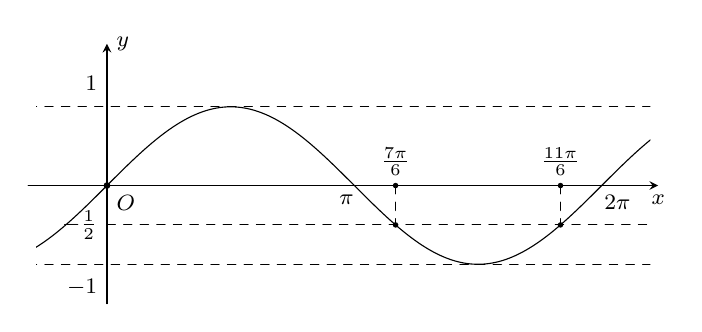
\begin{tikzpicture}[scale=1,font=\footnotesize,line join=round,line cap=round,>=stealth]
					\def\xmin{-1} \def\xmax{7} \def\ymin{-1.5}  \def\ymax{1.8}
					\draw[->] (\xmin,0)--(\xmax,0) node [below]{$x$}; 
					\draw[->] (0,\ymin)--(0,\ymax)  node [right]{$y$};
					\node at (0,0) [below  right]{$O$};
					\clip (\xmin+0.1,\ymin+0.1) rectangle  (\xmax-0.1,\ymax-0.1);
					\draw[smooth,samples=400,domain=\xmin:\xmax] plot (\x,{sin (\x r)}); 
					\draw[dashed] (\xmin,1)--(\xmax,1) 
						(\xmin,-1)--(\xmax,-1); 
					\foreach \x in  {-2*pi,-1.5*pi,-pi,-0.5*pi,0}
						{\draw[fill]  (\x,sin \x*180/pi) circle (1pt);}
					 \draw[dashed] (0,-0.5) node[left]{$-\frac{1}{2}$}--(7,-0.5)
						(7*pi/6,0) node[above]{$\frac{7\pi}{6}$}--(7*pi/6,-0.5) 
						(11*pi/6,0)  node[above]{$\frac{11\pi}{6}$}--(11*pi/6,-0.5);
					 \fill (7*pi/6,0) circle (1.0pt)
						(11*pi/6,0) circle  (1.0pt)
						(7*pi/6,-0.5) circle  (1.0pt)
						 (11*pi/6,-0.5) circle (1.0pt);
					\node at (0,1.3) [left]{$1$}; 
					\node  at (0,-1.3) [left]{$-1$};
					\node at  (pi-0.1,0) [below]{$\pi$};
					\node  at (2*pi+0.2,0) [below]{$2\pi$};
				\end{tikzpicture}
		\end{center}
		Dựa vào đồ thị trên đoạn $[0;2\pi]$ ta  có $s\leq-\dfrac{3}{2}$ khi $3\sin x\leq-\dfrac{3}{2}$ hay $\sin x\leq-\dfrac{1}{2}$.\\
	 Suy ra $\dfrac{7\pi}{6}\leq x\leq\dfrac{11\pi}{6}$ nên do đó $\dfrac{7}{3}\leq t\leq\dfrac{11}{3}$.}
\end{ex}

% nguồn: Ok_TuanLuan_Toan11_Lan2
\begin{ex}%[1D1V4-8]%[ma:6b4d244b]
	Huyết áp là áp lực máu cần thiết tác động lên thành động mạch nhằm đưa máu đi nuôi dưỡng các mô trong cơ thể. Nhờ lực co bóp của tim và sức cản của động mạch mà huyết áp được tạo ra. Giả sử huyết áp của một người thay đổi theo thời gian được cho bởi công  thức $p(t)=120+15\cos150\pi t$. Trong đó $p(t)$ là huyết áp tính theo đơn vị mmHg (milimét thuỷ ngân) và thời gian $t$ tính theo đơn vị phút.
	\begin{enumerate}
		\item Chứng minh $p(t)$ là một hàm số tuần  hoàn.
		\item Huyết áp cao nhất và huyết áp thấp nhất lần lượt được gọi là huyết áp tâm thu và huyết áp tâm trương. Tìm chỉ số huyết áp của người đó, biết rằng chỉ số huyết áp được viết  là huyết áp tâm thu/huyết áp tâm trương.
	\end{enumerate}
	\loigiai{ 
		\begin{enumerate}
			\item Hàm số $p(t)$ có tập xác định là $\mathbb{R}$.\\ 
			 Với mọi $t\in\mathbb{R}$, ta có $t\pm\dfrac{1}{75}\in\mathbb{R}$ và
			 $$p\left(t+\dfrac{1}{75}\right)=120+15\cos\left(150\pi t+2\pi\right)=120+15\cos150\pi t=p(t).$$
			Do đó  $p(t)$ là một hàm số tuần hoàn.
			\item Vì $-1\leq \cos150\pi t\leq 1$ với mọi  $t\in\mathbb{R}$ nên $105\leq p(t)\leq 135$ với mọi $t\in\mathbb{R}$.\\
			Vậy chỉ số huyết áp của người đó là  $135/105$.
	\end{enumerate}}
\end{ex}
